\chapter{基于多模态特征融合的锚点定位点云配准}
\thispagestyle{others}
\pagestyle{others}
\xiaosi

    \section{本章引言}
    点云中广泛存在可重复且模糊的结构,例如地板、墙壁和天花板都是平面。这些可重复且不明确的结构信息将在很大程度上影响特征的独特性、差异性。因此,只考虑点云结构信息的神经网络预测出来的对应关系中包含大量的离群值。如何提高点云特征的区分度是当前点云配准方法的主要研究方向。

    在早期研究阶段,大多数方法要么对几何结构进行充分的发掘和利用,要么参考图像配准方法开发新的配准框架,往往忽略了来自图片的纹理信息。二维图像虽然缺乏距离和角度等立体空间信息,但是其提供的颜色纹理等内容是人类理解世界的重要组成部分。近年来在3D目标检测和位置识别等领域越来越多的研究人员考虑将图像信息与点云信息融合起来。多模态信息融合的基本理论是利用模态信息间的互补性实现信息的相互补充提高特征的鲁棒性。就点云和图像而言,点云数据缺乏颜色信息和纹理信息但是对物体与环境的拓扑结构有着良好的表示,图像数据便能够作为有效的补充数据对点云数据进行补充。

    % 文献\cite{FPointNet}和文献\cite{F-ConvNet}将点云和图像进行拼接融合,首先通过标准的2D CNN特征提取器提取图像特征并于点云拼接,然后使用类似PointNet的模块进行回归分割和筛选每个点。
    % 相比之下,更多的研究同时完成了这一任务。
    文献\cite{9156790, 7780605}通过用逐点的2D分割特征增强3D坐标来进行数据级融合;文献\cite{8100174, 8594049}通过简单的拼接或特定模块实现来自单个网络的2D和3D表示的特征级融合。与仅使用激光雷达的方法不同,这种方法在单点云模式下不断更新更复杂的设计模型和更合适的训练方案,多模态替代方案努力利用更多样化的信息,并显示出巨大的潜力。

    尽管使用多模态的方法来进行特征提取受到越来越多的研究者的青睐,但是随之带来的挑战是不同模态之间存在着模态差异,如何更好的融合来自多种模态的信息是重点的研究方向。据调查发现,在3D目标检测的同行研究中,虽然研究人员期望这两种传感器的组合能够提供更好的性能,但事实证明,大多数最先进的3D物体探测器仅使用激光雷达作为输入。这表明如何有效地融合来自这两个传感器的数据仍然具有挑战性。
    虽然激光雷达点云和RGB图像具有互补的信息,但是由于两种模态的数据存在较大的域间隙,实现信息的互补并不容易。
    % 同时,当前算法往往使用卷积神经网络提取图像特征之后,将像素特征与原始点云进行简单拼接并输入点云骨干网络以完成特征融合,这进一步限制了融合效果。

    这种差距的出现主要由三方面造成:(1)点云和图像特征提取的网络之间存在较大差异,用于提取点云特征的网络往往针对点云数据的无序性,不规则性和稀疏性设计,而图像特征提取网络主要利用卷积对图像的结构和纹理信息进行提取,因此两种模态数据的特征之间存在着较大鸿沟,导致了融合过程中信息的丢失。(2)当前算法往往使用卷积神经网络提取图像特征之后,将像素特征与原始点云进行简单拼接并输入点云骨干网络以完成特征融合,这进一步限制了融合效果。这使得不同模态特征的相关性被忽略了,关键信息没有有效的突出。(3)数据增强技术被广泛应用于各种任务当中,但是对于多模态融合来说这种简单的机制可能不会有效的提高算法性能,这主要是由于对多模态而言对齐两种模态的数据是非常重要的,通过旋转平移等数据增强操作往往会造成模态间数据的错位。

    综上所述,本章为了提高点特征的区分度设计了一个点云图像融合的点云配准框架。提出了一个对齐模块将数据增强后的两种模态数据进行像素与超点间的对齐。提出一种新的多模态融合方法,先后在模态无关和模态相关两个子空间对点云特征和图像特征进行融合,减少模态间的域间隙和信息丢失。

    % 现有的最先进的点描述符仅依赖于结构信息,忽略了纹理信息。然而,纹理信息对于我们人类区分场景部分是至关重要的。本文提出了一种同时考虑结构和纹理信息的多模态融合方法来生成点云配准描述子。
    % 具体而言,设计了一种新的注意力融合模块,用于提取加权纹理信息,用于描述符提取。本文进一步解释了注册任务中的深度学习。在3DMatch、3DLoMatch和KITTI上的综合实验表明,多模态融合描述子达到了最先进的精度,提高了描述子的显著性。


    % 三维点描述符的特殊性决定了这些基于描述符的配准方法的性能。
    % 目前大多数3D描述符利用结构信息来描述点[1,5,12,20]。
    % 然而,点云中广泛存在可重复且模糊的结构,例如地板、墙壁和天花板都是平面(如图1所示)。这些可重复且不明确的结构信息将在很大程度上影响描述符的独特性。因此,通过比较仅结构的点描述符估计的对应关系包含显著的异常值。现有已发表的文献[1,5,12]已经证明了这种现象,当inlier阈值增加到0.2时,特征匹配召回率下降了很多。
    % 为了提高点描述子的独特性,提出了一种新的多模态融合方法,通过融合点云的结构信息和对应图像的纹理信息来学习三维点描述子。我们的动机在于,当我们观看一个场景时,我们通常会同时考虑纹理和结构,并区分两个部分——例如,红色的墙壁(Ip)和黄色的地板(Iq)(如图1所示)。
    % 具体来说,我们的多模态融合方法是基于FCGF[5]的编码器和解耦器架构。受变压器[22]的启发,在编码器模块之后,开发了一种新的交叉注意模块来提取每个点的加权纹理信息。然后,我们将纹理和结构信息连接起来,并将它们馈送到解耦器模块中进行最终的描述符学习。
    % 本文的主要贡献可以概括为:•提出了一种新的多模态融合方法来学习具有纹理和结构信息的三维点描述符。我们的方法将提高描述符的独特性。
    % •综合实验表明,所提出的多模态融合描述子在室内和室外数据集上都达到了最先进的性能。//IMFNet

    % 在本文中,我们提出了两种新技术:反演几何相关的增强(例如旋转),以实现激光雷达点和图像像素之间的精确几何对齐,以及LearnableAlign,利用交叉注意动态捕获融合过程中图像和激光雷达特征之间的相关性。基于InverseAug和LearnableAlign,我们开发了一系列通用的多模态3D检测模型,命名为DeepFusion,它比以前的方法更准确。

    % 文献中用于融合激光雷达和相机的现有方法大致遵循两种方法(图1):它们要么在早期阶段融合特征,例如用相应的相机特征装饰激光雷达点云中的点[34,36],要么使用中级融合,在特征提取后将特征组合在一起[13,17]。

    % 在这两种方法中最大的挑战之一是找出激光雷达和相机功能之间的对应关系。为了解决这个问题,我们提出了两种方法:InverseAug和LearnableAlign来实现有效的中层融合。InverseAug反演几何相关的数据增强,然后使用原始相机和激光雷达参数将两种模式关联起来。LearnableAlign利用交叉注意动态学习激光雷达特征与其对应的相机特征之间的相关性。这两种技术简单、通用、高效。基于PointPillars[16]和CenterPoint[44]等流行的3D点云检测框架,InverseAug和LearnableAlign可以帮助相机图像以边际计算成本(即只有一个交叉注意层)有效地与激光雷达点云对齐。当融合对齐的多模态特征时,摄像机信号具有更高的分辨率,显著提高了模型的识别和定位能力。这些优点尤其有利于远距离目标检测。
    % 我们开发了一系列名为deepfusion的多模态3D检测模型,其优势在于:(1)可以端到端训练,(2)是与许多现有的基于体素的3D检测方法兼容的通用构建块。DeepFusion作为一个插件,可以很容易地应用于大多数基于体素的3D检测方法,如PointPillars[16]和CenterPoint[44]。
    % 我们的大量实验表明(1)有效的深度特征对齐是多模态三维物体检测的关键,(2)通过我们提出的InverseAug和LearnableAlign提高对齐质量,DeepFusion显著提高了检测精度,(3)与单模态基线相比,DeepFusion对输入破坏和分布不均匀的数据更加稳健。
    % 在Waymo开放数据集上,DeepFusion改进了几个流行的3D检测模型,如PointPillars [16], CenterPoints[44]和3D- man[43],分别提高了6.7,8.9和6.2 LEVEL 2 APH。我们在Waymo开放数据集上取得了最先进的结果,DeepFusion在验证集上比之前最好的多模态方法pointaug[36]提高了7.4 Pedestrian LEVEL 2 APH。这一结果表明,我们的方法能够有效地结合激光雷达和相机模式,其中最大的改进来自于对远距离目标的识别和定位。
    % 我们的贡献可以概括为三个方面:•据我们所知,我们是第一个系统地研究深度特征对齐对3D多模态检测器的影响的人;•我们提出InverseAug和LearnableAlign来实现深度特征级对齐,从而实现准确和鲁棒的3D物体检测器;•我们提出的模型deepfusion在Waymo开放数据集上实现了最先进的性能。//deepfusion

    % 为了解决这一问题,我们提出了一个新的框架,即用于多模态3D目标检测的对比增强变压器(CAT-Det)。具体来说,CATDet采用了由Pointformer (PT)分支、Imageformer (IT)分支和Cross-Modal Transformer (CMT)模块组成的双流结构。PT、IT和CMT联合编码了表示对象的模内和模间长程上下文,从而充分探索了用于检测的多模态信息。此外,我们提出了一种有效的单向多模态数据增强(OMDA)方法,通过点级和对象级的层次对比学习,仅通过增强点云即可显著提高精度,而无需复杂地生成两种模态的配对样本。在KITTI基准上进行的大量实验表明,CAT-Det达到了新的最先进水平,突出了其有效性。

    % 为了解决上述问题,本文提出了一种新的多模态三维目标检测框架,即对比增强变压器检测器(CA T-Det)。它采用双流结构,由Pointformer (PT)分支、Imageformer (It)分支和Cross-Modal Transformer (CMT)模块组成。与pointnet++和cnn不同的是,PT和IT分支都拥有较大的接受域,分别能够在点云和图像中捕获丰富的全局上下文信息,加强硬样本的特征。随后,CMT模块进行跨模态特征交互和多模态特征组合,通过整体学习的细粒度权重充分强调两种模态提取的基本线索。PT、IT和CMT的集成充分编码了模态内和模态间的长期依赖关系,从而提高了检测性能。此外,我们提出了一种单向多模态数据增强(OMDA)方法,该方法通过分层对比学习,仅在点云模态上执行即可实现有效的增强。
    % 综上所述,本文的主要贡献是:(1)我们提出了一种新的CA T-Det框架,用于多模态三维物体检测,它包含一个点前分支、一个图像前分支和一个跨模态转换器模块。据我们所知,这是将变压器结构应用于给定任务的第一次尝试。(2)我们提出了一种单向数据增强的多模态三维目标检测方法,通过分层对比学习,仅通过增强点云就能显著提高精度,从而避免了两种模态成对样本的复杂生成。(3)我们在KITTI测试集上实现了所有三个类别的最新最先进的mAP,并与已发表的同类进行了比较,并证明了其在检测硬物体方面的优势。

    \section{基于多模态特征融合的锚点定位点云配准方法}
    为了更有效的提高源点云和目标点云相似非重叠区域特征间的特征差异性,本章提出了一个基于多模态特征融合点云配准新框架,整个方法遵循图\ref{fig:4-1}所示的基于多模态融合的点云配准新框架结构。

    \vspace{-0.1cm}
    \begin{figure}[h]
        \centering
        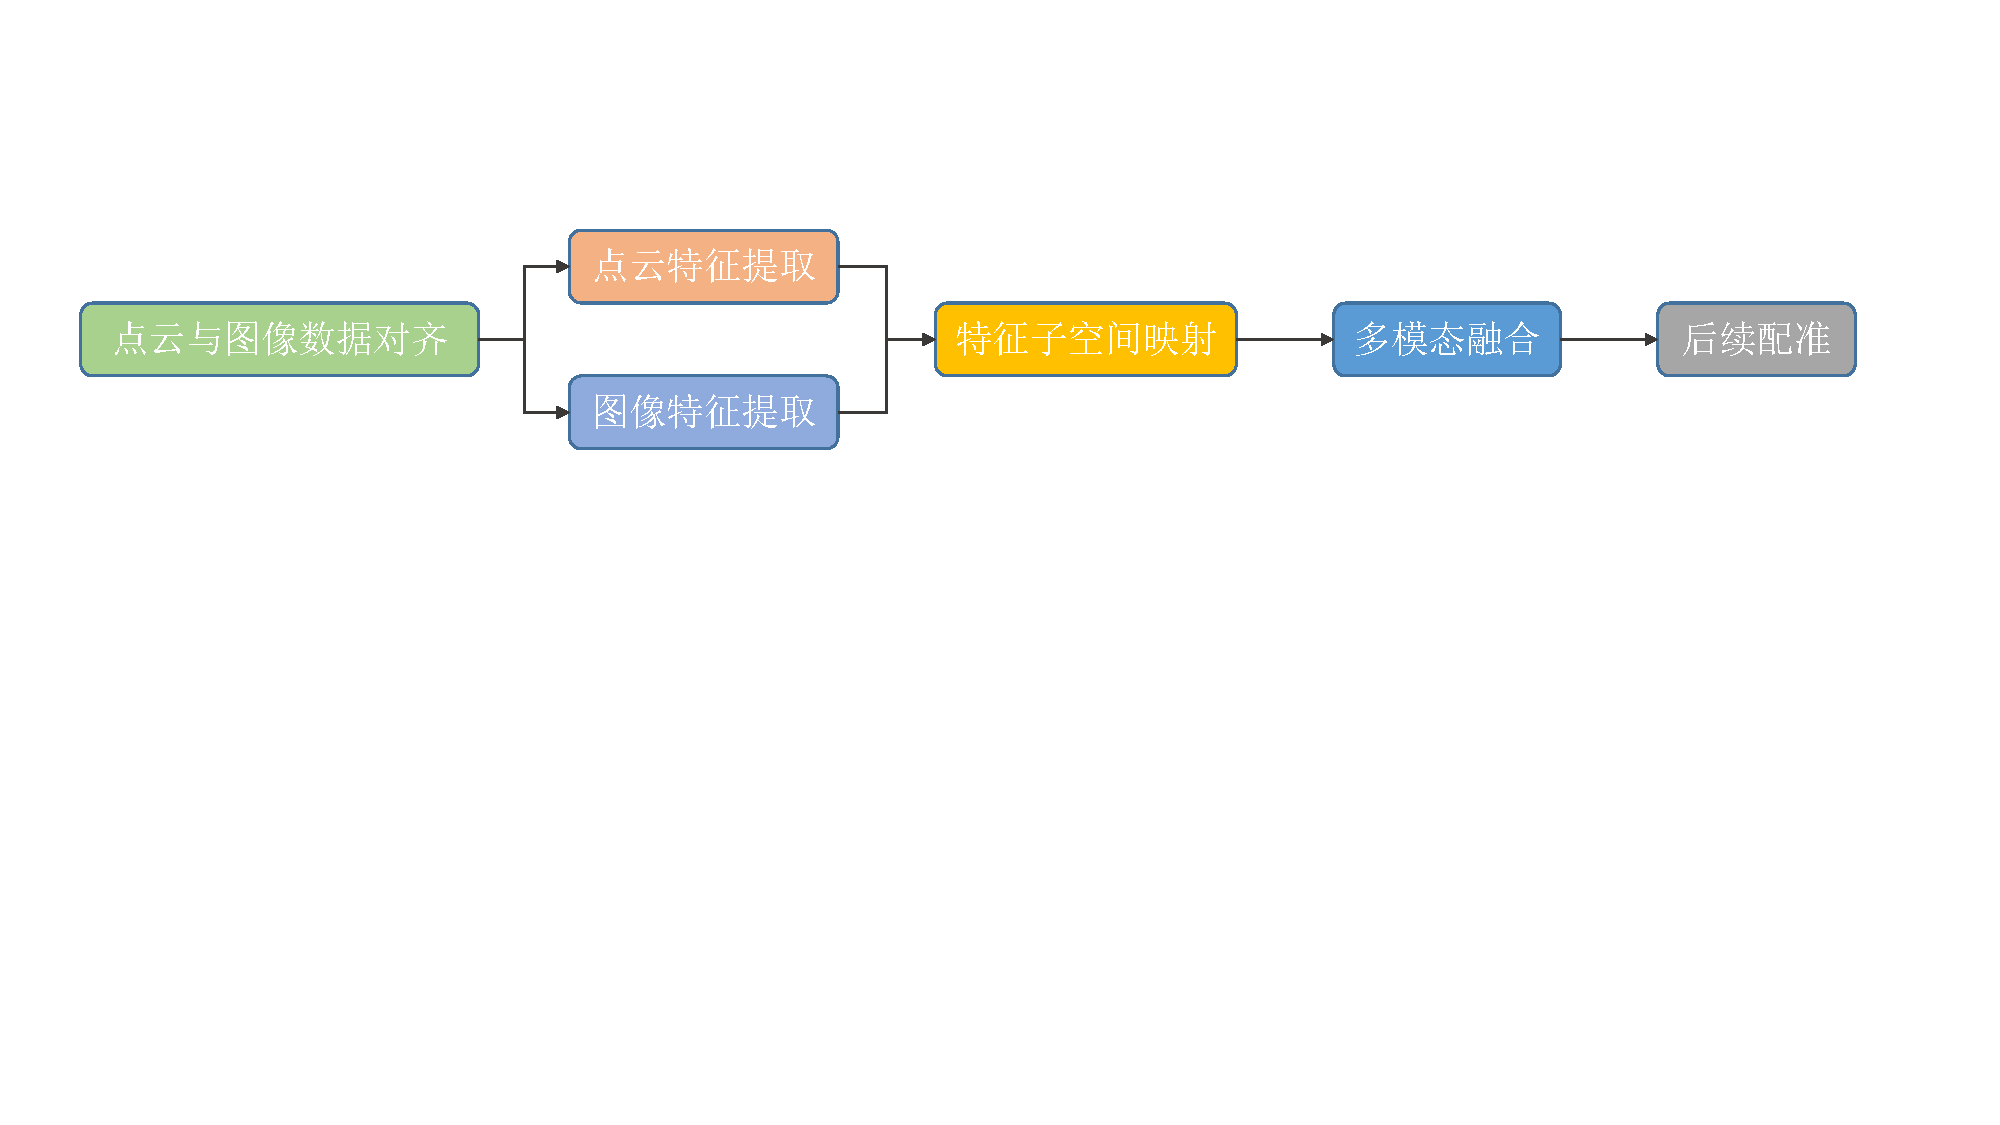
\includegraphics[width = \textwidth]{my/figure/4-1.pdf}
        % \captionsetup{margin = {1.6cm,1.6cm}}
        \bicaption[\xiaosi 第四章方法示意图]{\wuhao 本方法示意图}{\wuhao Schematic diagram of the method}
        \label{fig:4-1}
    \end{figure}
    \vspace{-0.35cm}

    图\ref{fig:4-2}展示了整个方法的示意图。该方法主要包括三个步骤:(1)在特征提取之前进行数据对齐,将点云和对应图像间的空间位置对齐即将点云中点的坐标投影至图像中,寻找点与像素之间的对应关系;(2)从点云中提取出超点的局部几何特征,并从各自对应的图像中提取二维纹理特征;(3)最后使用基于注意力机制的融合模块,将点云中的超点的特征与对应像素的纹理特征相融合,得到融合特征。
    随后操作与第三章中的方法一致,通过融合后的特征寻找具有显著特征且位于重叠区域的锚点,然后利用自注意力和交叉注意力机制对点云的几何结构特征进行编码,接着通过迭代优化更新显著超点与超点特征,最终将超点匹配扩充为点匹配并估计变换矩阵。

    基于多模态特征融合的锚点定位点云配准方法的重点在强调点云和图像间数据的对齐作为多模态融合的前置操作,经过对齐模块能够寻找到点云中的点与对应图像中像素的对应关系,相比于使用全局融合,这种融合方法是能够更加准确的有效的融合点的颜色纹理信息。许多以前的方法都没有在多模态融合之前进行额外的操作,这使得他们的融合效果受到限制;同时该方法在融合之前将模态数据投影到两个子空间中,通过减少域间隙融合两种不同模态的数据能够减少冗余信息对特征的干扰,使得多模态融合的效果更好。

    \vspace{-0.1cm}
    \begin{figure}[h]
        \centering
        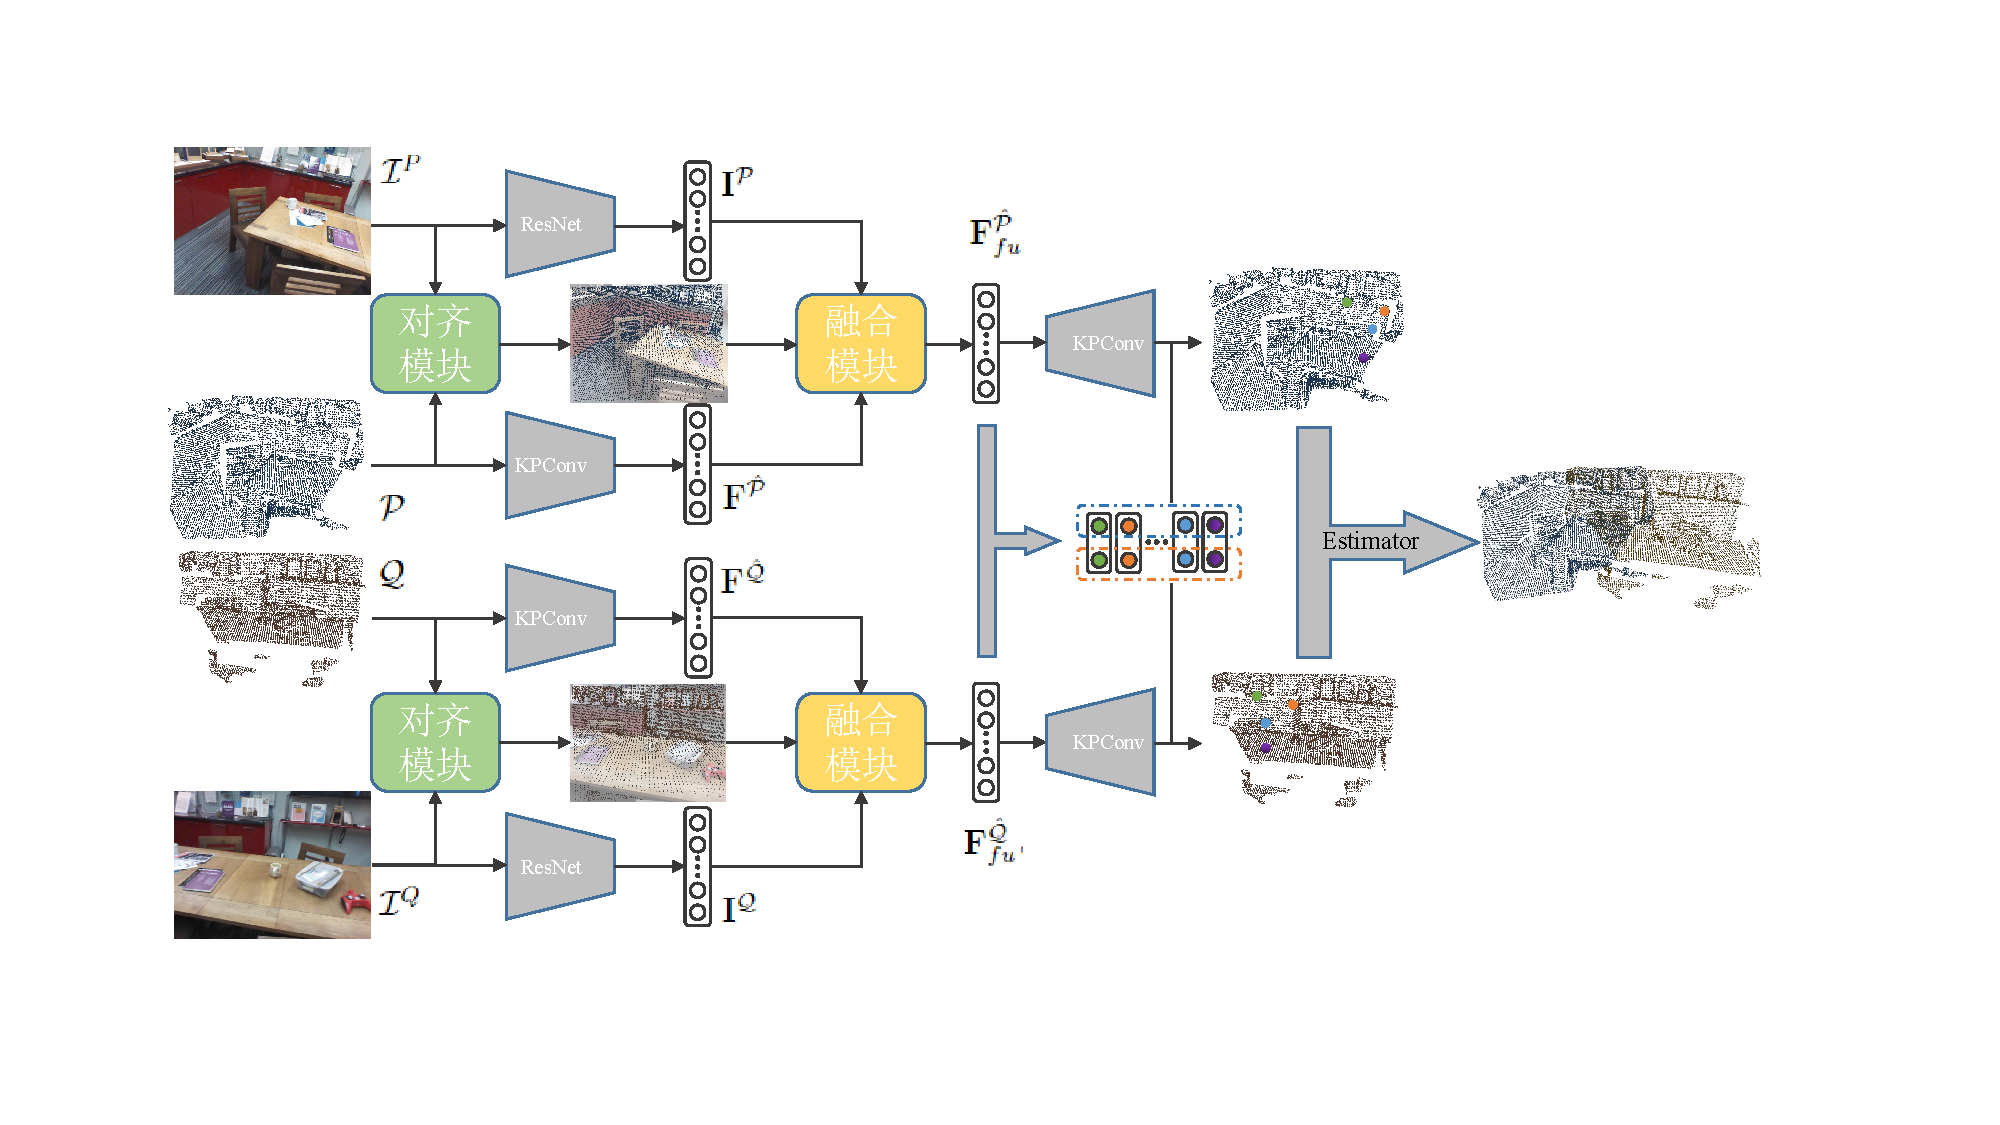
\includegraphics[width = \textwidth]{my/figure/4-2.pdf}
        % \captionsetup{margin = {1.6cm,1.6cm}}
        \bicaption[\xiaosi 第四章方法框架图]{\wuhao 本方法框架图}{\wuhao Overview of the proposed registration method}
        \label{fig:4-2}
    \end{figure}
    \vspace{-0.35cm}

    该方法的贡献如下:(1)对于点云和图像模态,使用对齐模块将点云和图像之间的数据对齐,具体而言将点云投影至二维平面并与图像对齐,寻找到超点与像素之间的一种一对多的对应关系;(2)在多模态融合之前,将投影两种模态的数据到正交的子空间,并先后融合两种模态数据学习跨模态的信息。

    \subsection{对齐模块}
    为了训练图像和点云数据,本文提出了一个融合模块,用于将图像的纹理颜色和点云的几何结构进行融合。因此,需要找到点云中的点和图像中的像素之间的对应关系。从三维空间到二维图像有一个成像过程,本模块通过将三维点云投影到二维图像,以便精确的寻找到点和像素之间的映射关系,促进后续两种模态特征的融合。对于源点云$\mathcal{P}$和源点云对应的图像$\mathcal{I}^\mathcal{P}$而言,它们之间的成像过程可以由公式(4-1)表示:
    \begin{equation}
        \mathcal{I}^\mathcal{P} = \mathbf{K}_{in} \mathbf{T}_{ex} \mathcal{P}
    \end{equation}
    式中,$\mathbf{K}_{in}$表示相机的内参矩阵;$\mathbf{T}_{ex}$表示相机的外参矩阵。对于未经过数据增强的点云和图像而言外参矩阵$\mathbf{T}_{ex}$为4阶单位矩阵,$\mathbf{K}_{in}$则与相机本身相关且不受到数据增强的影响。\par

    一种处理方式是不对点云数据进行数据增强处理,然而这种简单的处理方法会使模型在训练过程中陷入过拟合。本方法为了避免模型过拟合依旧采用随机旋转和增强噪音等策略。然而这时如果不采用额外的处理,依旧使用4阶单位矩阵作为外参矩阵$\mathbf{T}_{ex}$,那么点云的投影和图像之间将会存在偏差,这将导致点的颜色信息被错误的融合了,进一步到整体模型性能的下降。文献\cite{Deepfusion}指出数据增强对模型的促进作用将会随着随机旋转角度的增大而下降。这也进一步表明在特征融合之前对齐点云和图像两种模态的数据是至关重要的。

    为了解决数据增强带来的对齐偏差问题,本文提出了一个模态对齐模块。为了使重定位可行,对点云进行数据增强后,首先保存数据增强相关参数比如旋转角度。在对齐阶段,它将这些数据增强进行反转,得到输入点云中的三维空间点的原始坐标,然后在相机空间中找到其对应的二维坐标。由于本方法采用的是又粗到细的配准框架,即在提取点云特征过程中将点云下采样为超点。超点与原始点之间存在一对多的关系,而原始点与像素存在一对一的关系,因此最终本模块将得到超点与像素之间的一对多的对应关系。这种对应关系表示一个超点是图像中某块区域。最终,本节将得到超点与像素之间的对应关系矩阵$\mathbf{C}^{\hat{P}} \in \mathbb{R}^{N' \times L}$。同理本节会得到目标点云与其图像间的对应关系$\mathbf{C}^{\hat{Q}} \in \mathbb{R}^{M' \times L}$。

    % 当前许多将点云和图像数据融合的多模态方法往往通过图像特征提取器提取图像特征之后,利用图像特征修饰原始点云,再将修饰后的点云输入点云特征提取其中提取后续任务所需要的点云特征。然而这种方法忽略了图像特征提取器与点云特征提取器之间的域间隙,这种前融合方式并没有对图像和点云的特点进行分析导致融合后的特征并不能有效提高最终性能。
    % 综上,本章采用一种后融合的方式来深度融合点云和图像,分别通过点云和图像的特征提取器提取点云特征和图像特征;然后将两种模态的特征融合;最后将融合后的特征通过基于显著锚点几何嵌入的点云配准框架的其他组件得到最终的配准结果 。
    % 与之前的方法相比本章的融合方法能够有效缓解模态间的域间隙问题。然而,缺点也很明显,与输入级装饰相比,在深度特征层面上,将图像特征与点云特征对齐变得并不直接。例如,两种模态的异构数据增强导致的不准确对齐可能对融合阶段构成潜在挑战。

    \subsection{多模态特征提取}
    该方法的另一模块是多模态特征提取,而多模态特征的提取的核心是从点云和是图像当中提取出能够很好地代表点云局部结构和图像纹理信息的特征。本研究将源点云和目标点云输入到KPConv网络中,该网络能过够在提取特征的同时将点云下采样为超点。另一方面,本方法将对应的图像输入到用于提取像素特征的标准的ResUNet骨干网络中。选择ResUNet主要是因为可以加载该网络的最流行的预训练模型。这种由大数据集训练而来预训练模型,能够使网络起初就拥有良好的图像特征,同时使网络在训练过程中更加稳定。

    具体的网络结构遵循CofiNet使用KPConv稀疏卷积网络。输入源点云$\mathcal{P} \in \mathbb{R}^{N \times 3}$和目标点云$\mathcal{Q} \in \mathbb{R}^{M \times 3}$,输出$\mathbf{F}^{\hat{\mathcal{P}}} \in \mathbb{R}^{N' \times d}$和$\mathbf{F}^{\hat{\mathcal{Q}}} \in \mathbb{R}^{M' \times d}$。
    输入是源点云和目标点云对应的图像
    $\mathcal{I}^P \in \mathbb{R}^{W \times H \times 3}$ 和
    $\mathcal{I}^Q \in \mathbb{R}^{W \times H \times 3}$,
    输出是其特征
    $\mathbf{I}^{\mathcal{P}} \in \mathbb{R}^{L \times d}$ 和
    $\mathbf{I}^{\mathcal{Q}} \in \mathbb{R}^{L \times d}$。其中图像特征的维度$L = H \times W$。

    \subsection{融合模块}
    在经过模态数据的对齐和多模态特征提取之后,本节将对不同模态的特征进行融合。首先将不同模态特征提取到的点云和图像特征投影到不同的子空间中捕获模态相关和模态无关的信息,以获得更全面的特征表示。不失一般性,以源点云为例。在得到点云特征$\mathbf{F}^{\hat{\mathcal{P}}}$和图像特征$\mathbf{I}^{\mathcal{P}}$之后,点云中第$k$个超点的特征以符号$\mathbf{F}^{\hat{\mathcal{P}}}(k)$表示,第$k$个超点在图像中的对应区域内所有像素的特征构成一个集合以符号$\{\mathbf{I}^{\mathcal{P}}(k)\}$表示。具体如图\ref{fig:4-3}所示,图中紫色点代表超点,而图像中的紫色区域代表该超点的对应区域。
    % $\{\mathbf{I}^{\hat{\mathcal{P}}}(k)\}$
    利用解耦器$\mathbf{E}^{P}_{ir}$和解耦器$\mathbf{E}^{P}_{co}$对$\mathbf{F}^{\hat{\mathcal{P}}}(k)$进行解码,将其映射到模态无关和模态相关两个子空间中。用$\mathbf{F}^{\hat{\mathcal{P}}}_{ir}(k)$和$\mathbf{F}^{\hat{\mathcal{P}}}_{co}(k)$分别表示点云的模态无关特征和模态相关特征。

    \vspace{-0.1cm}
    \begin{figure}[ht]
        \centering
        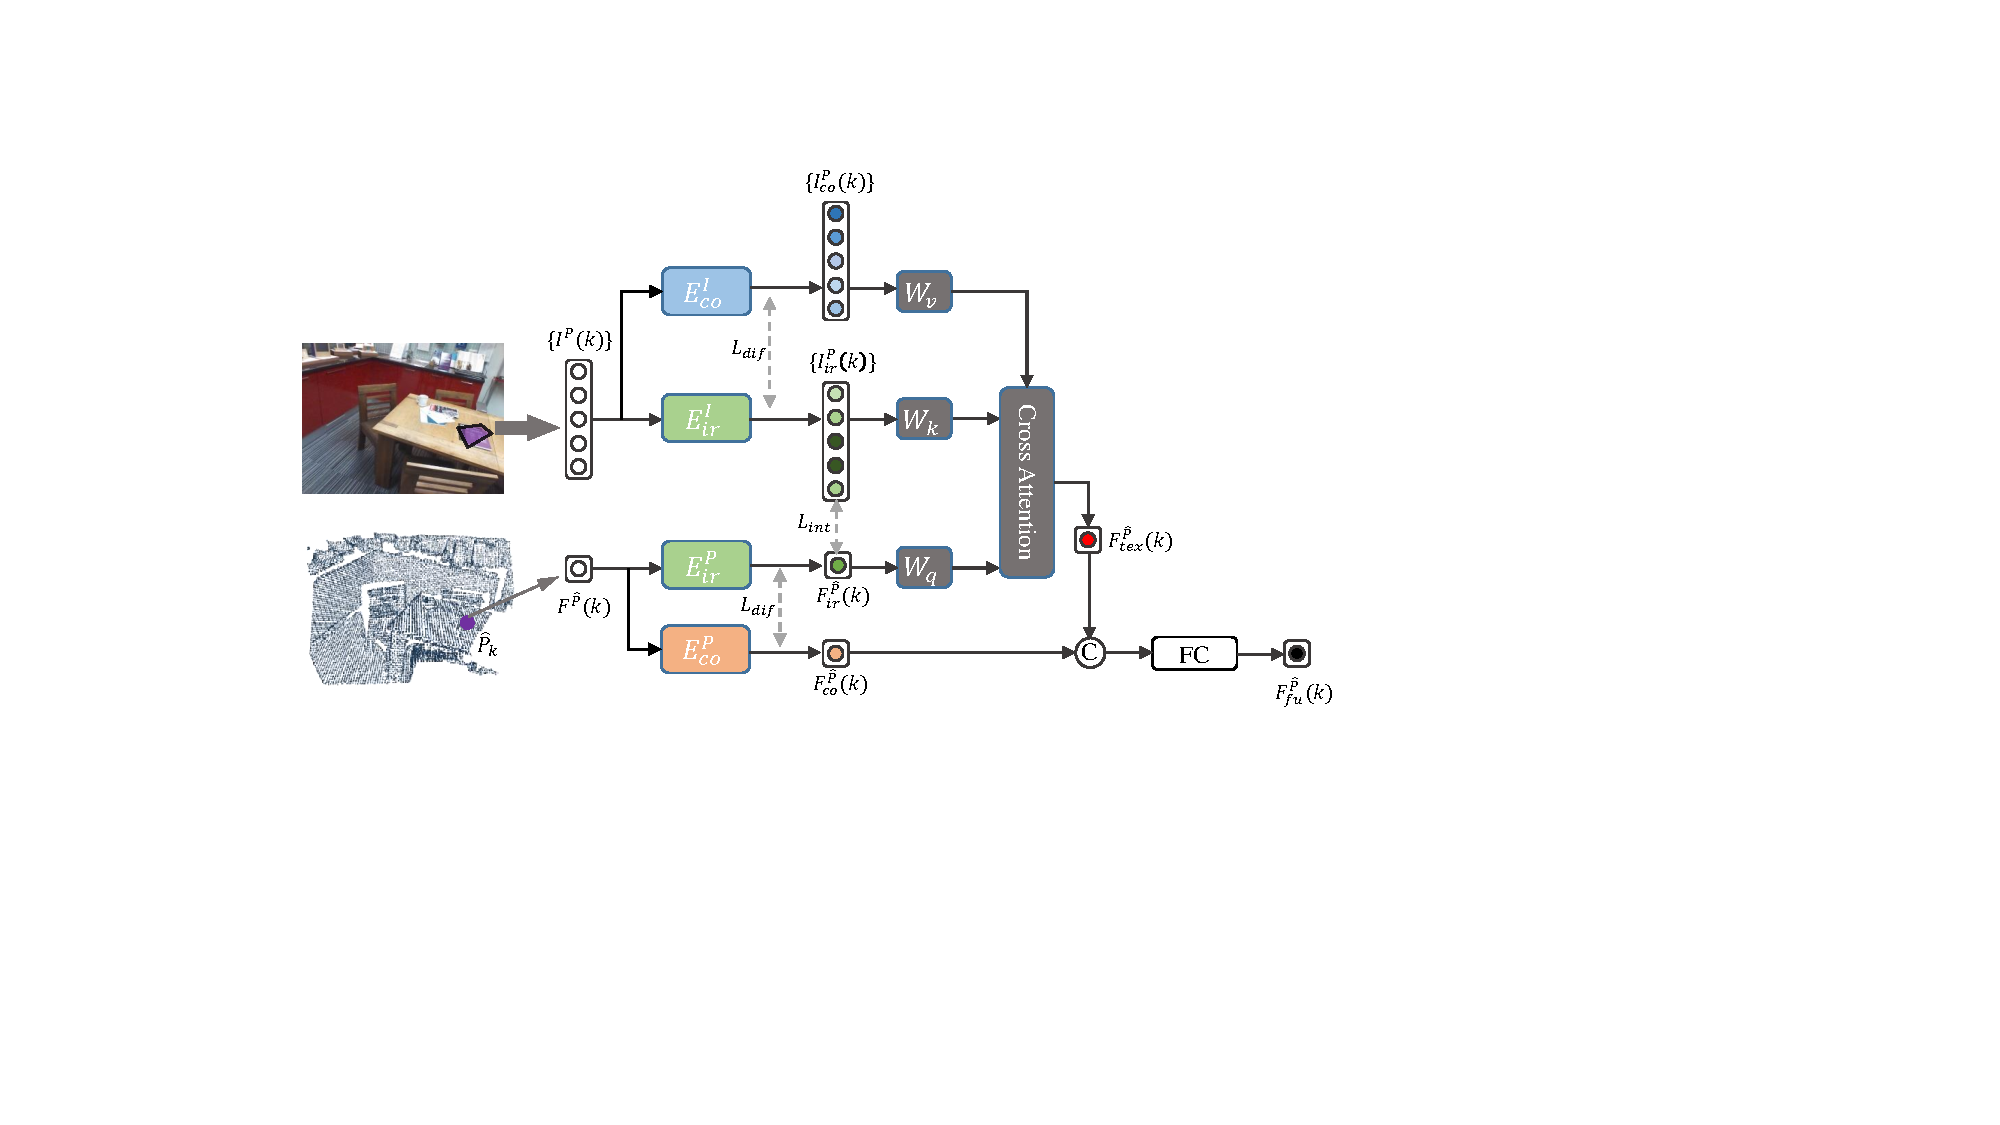
\includegraphics[width = \textwidth]{my/figure/4-3.pdf}
        % \captionsetup{margin = {1.6cm,1.6cm}}
        \bicaption[\xiaosi 特征融合模块流程图]{\wuhao 特征融合模块流程图}{\wuhao Flowchart of feature fusion module}
        \label{fig:4-3}
    \end{figure}
    \vspace{-0.35cm}

    类似的,利用解耦器$\mathbf{E}^{I}_{ir}$和解耦器$\mathbf{E}^{I}_{co}$将$\{\mathbf{I}^{\mathcal{P}}(k)\}$解码为图像模态无关特征$\{\mathbf{I}^{\mathcal{P}}_{ir}(k)\}$和图像模态相关特征$\{\mathbf{I}^{\mathcal{P}}_{co}(k)\}$。可用公式(4-2)表示上述解码过程:
    \begin{equation}
        \left\{
        \begin{aligned}
            \{{\mathbf{I}^{\mathcal{P}}_{ir}(k)}\} = \mathbf{E}^{I}_{ir}(\{\mathbf{I}^{\mathcal{P}}(k)\}) \\
            \{{\mathbf{I}^{\mathcal{P}}_{co}(k)}\} = \mathbf{E}^{I}_{co}(\{\mathbf{I}^{\mathcal{P}}(k)\}) \\
            \mathbf{F}^{\hat{\mathcal{P}}}_{ir}(k) = \mathbf{E}^{P}_{ir}(\mathbf{F}^{\hat{\mathcal{P}}}(k)) \\
            \mathbf{F}^{\hat{\mathcal{P}}}_{co}(k) = \mathbf{E}^{P}_{co}(\mathbf{F}^{\hat{\mathcal{P}}}(k))
        \end{aligned} \right.
    \end{equation}

    提取模态无关特征的目的在于提取潜在的公共特征,从而缩小不同模态之间的域间隙。在得到$\mathbf{F}^{\hat{\mathcal{P}}}_{ir}(k)$和$\{\mathbf{I}^{\mathcal{P}}_{ir}(k)\}$之后,本模块利用可学习矩阵$\mathbf{W}_q$和$\mathbf{W}_k$分别对两种模态无关特征进行映射后计算得到第$k$超点与它所对应图像区域像素的相似度矩阵$\mathbf{S}^{P}(k)$。具体来说,第$k$个超点与它的第$i$个像素的相似度分数$s^{P}(k,i)$可由公式(4-3)计算:
    \begin{equation}
        \begin{aligned}
            \mathbf{s}^{P}(k,i) = 
            (\mathbf{W}_q \mathbf{F}^{\hat{\mathcal{P}}}_{ir}(k))
            (\mathbf{W}_k \mathbf{I}^{\mathcal{P}}_{ir}(k,i))^\mathrm{T}
        \end{aligned}
    \end{equation}
    
    式中,$\mathbf{I}^{\mathcal{P}}_{ir}(k,i)$是第$k$个超点的第$i$个对应像素特征$\mathbf{I}^{\mathcal{P}}(k,i)$在模态无关子空间中的投影。随后$\{\mathbf{I}^{\mathcal{P}}_{co}(k)\}$经过$\mathbf{W}_v$的映射并结合相似度矩阵进行加权求和可以得到第$k$超点的纹理特征$\mathbf{F}^{\mathcal{P}}_{tex}(k)$:
    \begin{equation}
        \begin{aligned}
            \mathbf{F}^{\mathcal{P}}_{tex}(k) = \sum_i \mathbf{s}^{P}(k,i) \mathbf{I}^{\mathcal{P}}_{co}(k,i)
        \end{aligned}
    \end{equation}
    式中,$\mathbf{I}^{\mathcal{P}}_{co}(k,i)$第$k$个超点的第$i$个对应像素特征$\mathbf{I}^{\mathcal{P}}(k,i)$在模态相关子空间中的投影。相比于直接利用$\mathbf{F}^{\hat{\mathcal{P}}}(k)$与$\{\mathbf{I}^{\mathcal{P}}(k)\}$进行特征融合,上述方法由于在特征无关子空间中进行不同模态特征的查询,缩小了两种模态的域间隙减少了独有信息的影响。同理可以得到源点云中所有超点的纹理特征$\mathbf{F}^{\hat{\mathcal{P}}}_{tex}$。

    在得到超点的纹理特征$\mathbf{F}^{\mathcal{P}}_{tex}$之后,本文再将超点的模态相关特征$\mathbf{F}^{\hat{\mathcal{P}}}_{co}$与之在通道维度上拼接,并将其送入最后的映射层完成特征融合。可由公式(4-5)表示:
    \begin{equation}
        \mathbf{F}^{\hat{\mathcal{P}}}_{fu} = f(\mathbf{F}^{\hat{\mathcal{P}}}_{co} \oplus \mathbf{F}^{\hat{\mathcal{P}}}_{tex})
    \end{equation}
    式中,$f(\cdot)$表示映射层,由全连接层和激活函数构成。将$\mathbf{F}^{\mathcal{P}}_{tex}$和$\mathbf{F}^{\hat{\mathcal{P}}}_{co}$融合主要是为了避免两种模态独有信息的丢失。同理可以得到目标点云融合后的超点特征$\mathbf{F}^{\hat{\mathcal{Q}}}_{fu}$。

    \subsection{损失函数}
    为了使融合模块中的四个解耦器$\mathbf{E}^{I}_{ir}$、$\mathbf{E}^{I}_{co}$、$\mathbf{E}^{P}_{ir}$和$\mathbf{E}^{P}_{co}$达到设计要求。本文利用差异损失$\mathcal{L}_{dif}$和三元组损失$\mathcal{L}_{int}$分别监督同一模态特征和不同模态特征。
    \subsubsection{差异损失}
    差异损失主要是为了使同一模态的两种解码器能够捕获输入特征的不同方面的信息。通过解耦模态相关特征和模态无关特征之间存在一个正交约束。具体的,对于第$k$个超点的第$i$个像素特征在两个子空间的投影$\mathbf{I}^{\mathcal{P}}_{ir}(k,i)$和$\mathbf{I}^{\mathcal{P}}_{co}(k,i)$来说,理论上它们存在公式(4-6)的正交约束:
    \begin{equation}
        \Vert \mathbf{I}^{\mathcal{P}}_{ir}(k,i) (\mathbf{I}^{\mathcal{P}}_{co}(k,i))^\mathrm{T} \Vert^2_F = 0
    \end{equation}
    式中,$\Vert \cdot \Vert^2_F$表示Feobenius范数的平方。同时,这种约束对于第$k$个超点在两个子空间中的投影依旧成立。为此,本文使用的差异损失$\mathcal{L}_{dif}$如公式(4-7)所示:
    \begin{equation}
        \mathcal{L}_{dif} = 
        \sum_k (\Vert \mathbf{F}^{\hat{\mathcal{P}}}_{ir}(k) (\mathbf{F}^{\hat{\mathcal{P}}}_{co}(k))^\mathrm{T} \Vert^2_F) + 
        \sum_{k,i} (\Vert \mathbf{I}^{\mathcal{P}}_{ir}(k,i) (\mathbf{I}^{\mathcal{P}}_{co}(k,i))^\mathrm{T} \Vert^2_F)
    \end{equation}

    \subsubsection{三元组损失}
    模态无关特征指的是同一事物的结构纹理等信息不随表示形式的变化而变化的那部分。将点云和图像两种模态的特征同时投影至模态无关子空间中,得到每个模态自身的模态无关向量。模态间的损失函数的作用就是让不同模态的模态无关向量更加相似,这有助于通过一种模态特征查询另一种模态特征。本方法使用三元组损失函数监督两种模态在模态无关子空间中的投影。三元组损失在拉近锚点和正样本之间距离的同时,增加锚点与负样本之间的距离。具体而言,任一超点的模态无关特征和它对应像素的模态无关特征之间的距离要小于它与其他像素之间的特征距离;同时,对应像素集合中的特征距离要小于与其他像素之间的特征距离。因此,本文使用的三元损失$\mathcal{L}_{int}$如公式(4-8)所示:
    \begin{equation}
        \begin{aligned}
        \mathcal{L}_{int} = 
        \sum_{k,x} max(\lambda - 
        d(\mathbf{F}^{\hat{\mathcal{P}}}_{ir}(k), \{\mathbf{I}^{\mathcal{P}}_{ir}(k)\}) + 
        d(\mathbf{F}^{\hat{\mathcal{P}}}_{ir}(k), \{\mathbf{I}^{\mathcal{P}}_{ir}(x)\}))
        \\
        +\sum_{k,x} max(\lambda - 
        d(\mathbf{F}^{\hat{\mathcal{P}}}_{ir}(k), \{\mathbf{I}^{\mathcal{P}}_{ir}(k)\}) + 
        d(\mathbf{F}^{\hat{\mathcal{P}}}_{ir}(x), \{\mathbf{I}^{\mathcal{P}}_{ir}(k)\}))
        \end{aligned}
    \end{equation}
    式中,$\lambda$用于控制正负样本之间的距离;$(\mathbf{F}^{\hat{\mathcal{P}}}_{ir}(k), {\mathbf{I}^{\mathcal{P}}_{ir}(k)})$对应三元损失中的正样本对;$(\mathbf{F}^{\hat{\mathcal{P}}}_{ir}(k), {\mathbf{I}^{\mathcal{P}}_{ir}(x)})$和$(\mathbf{F}^{\hat{\mathcal{P}}}_{ir}(x), {\mathbf{I}^{\mathcal{P}}_{ir}(k)})$对应三元函数的负样本对。$d(\mathbf{F}^{\hat{\mathcal{P}}}_{ir}(x), {\mathbf{I}^{\mathcal{P}}_{ir}(y)})$表示超点$\mathcal{P}_x$与超点$\mathcal{P}_y$所对应像素集之间的距离和,由公式(4-9)定义:
    \begin{equation}
        \begin{aligned}
        d(\mathbf{F}^{\hat{\mathcal{P}}}_{ir}(x), \{\mathbf{I}^{\mathcal{P}}_{ir}(y)\}) =
        \sum_i -\Vert max(0, \mathbf{F}^{\hat{\mathcal{P}}}_{ir}(x) - \mathbf{I}^{\mathcal{P}}_{ir}(y,i)) \Vert^2
        \end{aligned}
    \end{equation}

    \section{实验结果与分析}
    \subsection{数据集预处理}
    本章采用的数据集3DMatch和3DLoMatch与第三章略有差别。在上一章所用数据集的基础上本章为每个点云配对了RGB图像数据。RGB图像数据来自于最原始的3DMatch数据集,每50张图像合成一个点云数据。为了减少时间花销,本方法没有使用全部的50张图片而是选择第一张图片用于多模态融合。同时,本方法记录了第一帧图片的相机位姿和相机内参并加入了数据集,以保证本章中的对其模块能够正常使用。至此,整个数据集的预处理完成,整个数据集由点云、图像和相机的内参外参矩阵组成。
    \subsection{3DMatch和3DLoMatch实验}
    在本节中,本文对多模态融合的点云配准任务在3DMatch和3DLoMatch上进行了实验分析。实验表明,通过融合图像特征本方法的点云配准方法能够达到较好水平。
    % 在表\ref{tab:4-1-1}、表\ref{tab:4-1-2}和表\ref{tab:4-1-3}中分别记录了本方法在3DMatch和3DLoMatch数据集上采样数为5000、2500、1000、500和250时的内点率、特征召回率和配准召回率的实验对比。
    如表\ref{tab:4-1-1}所示,本方法在内点率上远高于其他方法。尤其当采样数为250时,在3DMatch和3DLoMatch上比CoFiNet分别高了32.4\%和30.2\%。这表明本方法能够在相同情况下比其他方法能够更加有效的找到正确的点对应。\par
    \begin{table}[htp]
    \renewcommand{\arraystretch}{1}
    \centering
    \bicaption[\xiaosi 第四章方法与先进方法的内点率]{\wuhao 本方法与先进方法的内点率和匹配召回率的比较}{\wuhao Comparison of Inlier Ratio with advanced methods}\label{tab:4-1-1}
    \wuhao

    \begin{tabular}{lcccccccccc}
    \toprule[1.5pt]
    \multicolumn{1}{c}{\multirow{3}{*}{\songti\wuhao Sample}} 
    & \multicolumn{5}{c}{\songti\wuhao 3DMatch}
    & \multicolumn{5}{c}{\songti\wuhao 3DLoMatch}
    \\\multicolumn{1}{c}{}
    &\songti\wuhao 5000 &\songti\wuhao 2500 &\songti\wuhao 1000 &\songti\wuhao500 
    &\multicolumn{1}{c}{\songti\wuhao 250}           
    &\songti\wuhao 5000 &\songti\wuhao 2500 &\songti\wuhao 1000 &\songti\wuhao500 
    &\songti\wuhao 250

    \\ \hline

    \multicolumn{1}{c}{\wuhao PerfectMatch}
    & 36.0          & 32.5          & 26.4          & 21.5          & \multicolumn{1}{c}{16.4}          & 11.4          & 10.1          & 8.1           & 6.4           & 4.8
    \\
    \multicolumn{1}{c}{\wuhao FCGF}
    & 56.8          & 54.1          & 48.7          & 42.5          & \multicolumn{1}{c}{34.1}          & 21.4          & 20.0          & 17.2          & 14.8          & 11.6
    \\
    \multicolumn{1}{c}{\wuhao D3Feat}
    & 39.0          & 38.8          & 40.4          & 41.5          & \multicolumn{1}{c}{41.8}          & 13.2          & 13.1          & 14.0          & 14.6          & 15.0
    \\
    \multicolumn{1}{c}{\wuhao SpinNet}
    & 47.5          & 44.7          & 39.4          & 33.9          & \multicolumn{1}{c}{27.6}          & 20.5          & 19.0          & 16.3          & 13.8          & 11.1
    \\
    \multicolumn{1}{c}{\wuhao Predator}
    & 58.0          & 58.4          & \ul{57.1}    & \ul{54.1}    & \multicolumn{1}{c}{49.3}          & \ul{26.7}    & \ul{28.1}    & \ul{28.3}    & \ul{27.5}    & 25.8
    \\
    \multicolumn{1}{c}{\wuhao YOHO}
    & \ul{64.4}    & \ul{60.7}    & 55.7          & 46.4          & \multicolumn{1}{c}{41.2}          & 25.9          & 23.3          & 22.6          & 18.2          & 15.0
    \\
    \multicolumn{1}{c}{\wuhao CoFiNet}
    & 49.8          & 51.2          & 51.9          & 52.2          & \multicolumn{1}{c}{\ul{52.2}}    & 24.4          & 25.9          & 26.7          & 26.8          & \ul{26.9}
    \\

    \multicolumn{1}{c}{\wuhao Ours}
    & \textbf{71.9} & \textbf{78.5} & \textbf{83.0} & \textbf{84.8} & \multicolumn{1}{c}{\textbf{85.8}} & \textbf{41.4} & \textbf{47.0} & \textbf{52.9} & \textbf{55.5} & \textbf{57.1}
    
    \\ \bottomrule[1.5pt]
    \end{tabular}
\end{table}

    对于特征召回率而言,本方法虽然在3DMatch上的表现一般,在采样数为5000、2500和250时分别比最优模型低了0.2\%、0.3\%和0.4\%。但是如表\ref{tab:4-1-2}所示,本方法在3DLoMatch的表现都达到了最优性能,分别比次优模型高了4.5\%、4.4\%、4.1\%、4.3\%和4.2\%。这表明本方法相比于其他方法能够更好的在低重叠率情况下工作,能够使源点云和目标点云之间的点对应更多,从而达到RANSAC算法发挥最用的最低要求。\par
    \begin{table}[htbp]
    \renewcommand{\arraystretch}{1}
    \centering
    \bicaption[\xiaosi 第四章方法与先进方法的匹配召回率的比较]{\wuhao 本方法与先进方法的匹配召回率的比较}{\wuhao Comparison of Feature Matching Recall with advanced methods}\label{tab:4-1-2}
    \wuhao

    \begin{tabular}{lcccccccccc}
    \toprule[1.5pt]
    \multicolumn{1}{c}{\multirow{3}{*}{\songti\wuhao Sample}} 
    & \multicolumn{5}{c}{\songti\wuhao 3DMatch}
    & \multicolumn{5}{c}{\songti\wuhao 3DLoMatch}
    \\\multicolumn{1}{c}{}
    &\songti\wuhao 5000 &\songti\wuhao 2500 &\songti\wuhao 1000 &\songti\wuhao500 
    &\multicolumn{1}{c}{\songti\wuhao 250}           
    &\songti\wuhao 5000 &\songti\wuhao 2500 &\songti\wuhao 1000 &\songti\wuhao500 
    &\songti\wuhao 250

    \\ \hline

    \multicolumn{1}{c}{\wuhao PerfectMatch}
    & 95.0          & 94.3          & 92.9          & 90.1          & \multicolumn{1}{c}{82.9}          & 63.6          & 61.7          & 53.6          & 45.2          & 34.2
    \\
    \multicolumn{1}{c}{\wuhao FCGF}
    & 97.4          & 97.3          & 97.0          & 96.7          & \multicolumn{1}{c}{96.6}          & 76.6          & 75.4          & 74.2          & 71.7          & 67.3
    \\
    \multicolumn{1}{c}{\wuhao D3Feat}
    & 95.6          & 95.4          & 94.5          & 94.1          & \multicolumn{1}{c}{93.1}          & 67.3          & 66.7          & 67.0          & 66.7          & 66.5
    \\
    \multicolumn{1}{c}{\wuhao SpinNet}
    & 97.6          & 97.2          & 96.8          & 95.5          & \multicolumn{1}{c}{94.3}          & 75.3          & 74.9          & 72.5          & 70.0          & 63.6
    \\
    \multicolumn{1}{c}{\wuhao Predator}
    & 96.6          & 96.6          & 96.5          & 96.3          & \multicolumn{1}{c}{96.5}          & 78.6          & 77.4          & 76.3          & 75.7          & 75.3
    \\
    \multicolumn{1}{c}{\wuhao YOHO}
    & \textbf{98.2} & 97.6          & 97.5    & \ul{97.7}    & \multicolumn{1}{c}{96.0}          & 79.4          & 78.1          & 76.3          & 73.8          & 69.1
    \\
    \multicolumn{1}{c}{\wuhao CoFiNet}
    & \ul{98.1}    & \textbf{98.3} & \ul{98.1} & \textbf{98.2} & \multicolumn{1}{c}{\textbf{98.3}} & \ul{83.1}    & \ul{83.5}    & \ul{83.3}    & \ul{83.1}    & \ul{82.6}
    \\
    \multicolumn{1}{c}{\wuhao Ours}
    & 98.0          & \ul{98.0}    & \textbf{98.4} & \textbf{98.2} & \multicolumn{1}{c}{\textbf{98.3}}    & \textbf{87.6} & \textbf{87.9} & \textbf{87.4} & \textbf{87.4} & \textbf{86.8}
    
    \\ \bottomrule[1.5pt]
    \end{tabular}
\end{table}

    本方法进一步与各个先进方法在匹配召回率上做了对比。如表\ref{tab:4-1-3}所示,本方法在3DLoMatch和3DMatch数据集上的性能均达到了当前最优的性能。具体来说,在3DMatch上当采样数为5000、2500、1000、500和250时,本模型的新能分别比次优模型高了0.2\%、1\%、0.1\%、1.4\%和2.3\%;在3DLoMatch上则分别高出了2.5\%、3.3\%、6\%、6.4\%和7.5\%。这表明本方法生成的点对应关系能够有效的实现点云间的配准。同时可以注意到,本方法的性能的变化幅度远远低于其他方法,其他模型的性能随着采样数的减少有明显下降。这表明本方法能够有效提取空间一致性的点对应,即使在低重叠率的情况下,也能够通过少数高置信度的点对应恢复点云间的变换矩阵。这也表明通过融合图像特征,本模型受到的噪声影响更小,模型更加稳定。\par
    \begin{table}[ht]
    \renewcommand{\arraystretch}{1}
    \centering
    \bicaption[\xiaosi 本方法与先进方法的配准召回率的比较]{\wuhao 本方法与先进方法的配准召回率的比较}{\wuhao Comparison of registration recall rates of this method with advanced methods}\label{tab:4-1-3}
    \wuhao
    
    \begin{tabular}{lcccccccccc}
    \toprule[1.5pt]
    \multicolumn{1}{c}{\multirow{3}{*}{\songti\wuhao Sample}} 
    & \multicolumn{5}{c}{3DMatch}
    & \multicolumn{5}{c}{3DLoMatch}
    \\ \multicolumn{1}{c}{}
    &\songti\wuhao 5000 &\songti\wuhao 2500 &\songti\wuhao 1000 &\songti\wuhao500 
    &\multicolumn{1}{c}{\songti\wuhao 250}           
    &\songti\wuhao 5000 &\songti\wuhao 2500 &\songti\wuhao 1000 &\songti\wuhao500 
    &\songti\wuhao 250    

    \\ \hline

    \multicolumn{1}{l}{\wuhao PerfectMatch}
    & 78.4          & 76.2          & 71.4          & 67.6          & \multicolumn{1}{c}{50.8}          & 33.0          & 29.0          & 23.3          & 17.0          & 11.0
    \\
    \multicolumn{1}{l}{\wuhao FCGF}
    & 85.1          & 84.7          & 83.3          & 81.6          & \multicolumn{1}{c}{71.4}          & 40.1          & 41.7          & 38.2          & 35.4          & 26.8
    \\
    \multicolumn{1}{l}{\wuhao D3Feat}
    & 81.6          & 84.5          & 83.4          & 82.4          & \multicolumn{1}{c}{77.9}          & 37.2          & 42.7          & 46.9          & 43.8          & 39.1
    \\
    \multicolumn{1}{l}{\wuhao SpinNet}
    & 88.6          & 86.6          & 85.5          & 83.5          & \multicolumn{1}{c}{70.2}          & 59.8          & 54.9          & 48.3          & 39.8          & 26.8
    \\
    \multicolumn{1}{l}{\wuhao Predator}
    & 89.0          & 89.9    & \ul{90.6} & 88.5          & \multicolumn{1}{c}{86.6}          & 59.8          & 61.2          & 62.4          & 60.8          & 58.1
    \\
    \multicolumn{1}{l}{\wuhao YOHO}
    & \ul{90.8} & \ul{90.3} & 89.1          & \ul{88.6} & \multicolumn{1}{c}{84.5}          & 65.2          & 65.5          & 63.2          & 56.5          & 48.0
    \\
    \multicolumn{1}{l}{\wuhao CoFiNet}
    & 89.3          & 88.9    & 88.4          & 87.4          & \multicolumn{1}{c}{\ul{87.0}}    & \ul{67.5}    & \ul{66.2}    & \ul{64.2}    & \ul{63.1}    & \ul{61.0}
    \\
    \multicolumn{1}{l}{\wuhao Ours}
    & \textbf{91.0}    &\textbf{91.3}          & \textbf{90.7}    & \textbf{90.0}    & \multicolumn{1}{c}{\textbf{89.3}} & \textbf{70.0} & \textbf{69.5} & \textbf{70.2} & \textbf{69.5} & \textbf{68.5}
    \\
    \bottomrule[1.5pt]
    \end{tabular}
\end{table}

    本章同样使用加权奇异值分解法和局部到全局变换估计两种算法估计变换矩阵,表\ref{tab:4-3}的实验结果进一步验证了上述表述。本实验首先使用加权奇异值分解算法求解变换矩阵,其他模型要么不能达到合理的结果,要么性能严重下降。比如CoFiNet模型使用加权奇异值分解进行变换估计时比基于RANSAC的变换估计性能在3DMatch和3DLoMatch上分别下降了24.7\%和49.5\%。相比之下,本方法在3DMatch上的配准召回率达到了84.7\%仅比利用RANSAC得到的结果下降了5.3\%。在3DLoMatch上虽然性能下降了14.1\%,但是也接近了Predator方法性能。这得益于本方法能够有效找到可靠和分布良好的超点对应。当使用局部到全局配准进行变换估计时,本方法在3DMatch上的配准召回率达到90.6\%,3DLoMatch的配准召回率达到73.1\%,基本达到了其他模型使用RANSAC的结果。\par
    \begin{table}[ht]
    \renewcommand{\arraystretch}{1}
    \centering
    \bicaption[\xiaosi 在3DMatch和3DLoMatch上使用不同姿态估计器的配准结果]{\wuhao 在3DMatch和3DLoMatch上使用不同姿态估计器的配准结果}{\wuhao Registration results with different pose estimators on 3DMatch and 3DLoMatch}\label{tab:4-3}
    \wuhao

    \begin{tabular}{lccccccc}
    \toprule[1.5pt]
    \multirow{2}{*}{\songti\wuhao Model} 
    & \multirow{2}{*}{\songti\wuhao Estimator} 
    & \multirow{2}{*}{\songti\wuhao Sample} 
    & \multicolumn{2}{c}{\songti\wuhao RR(\%)}   
    & \multicolumn{3}{c}{\songti\wuhao Times(s)} \\
    
    & &
    &{\songti\wuhao 3DMatch} &{\songti\wuhao 3DLoMatch}
    &{\songti\wuhao Model}   &{\songti\wuhao Pose}    &{\songti\wuhao Total}
    
    \\ \hline
    {\songti\wuhao FCGF} &{\songti\wuhao RANSAC-50k} & 5000
    & 85.1          & 40.1          & 0.098   & 9.015   & 9.113   
    \\
    % {\songti\wuhao D3Feat} &{\songti\wuhao RANSAC-50k} & 5000
    % & 81.6          & 37.2          & 0.055   & 8.217   & 8.272   
    % \\
    {\songti\wuhao Predator} &{\songti\wuhao RANSAC-50k} & 5000
    & 89.0          & 59.8          & 0.079   & 15.434  & 15.513  
    \\
    {\songti\wuhao CoFiNet} &{\songti\wuhao RANSAC-50k} & 5000
    & \uline{89.3}    & \uline{67.5}    & 0.259   & 5.321   & 5.580   
    \\
    {\songti\wuhao Ours} &{\songti\wuhao RANSAC-50k} & 5000
    & \textbf{91.0} & \textbf{70.0} & 0.141   & 4.215   & 4.356   
    
    \\ \hline
    {\songti\wuhao FCGF} &{\songti\wuhao weighted SVD} & 250
    & 42.1          & 3.9           & 0.098   & 0.008   & 0.106   
    \\
    % {\songti\wuhao D3Feat} &{\songti\wuhao weighted SVD} & 250
    % & 37.4          & 2.8           & 0.055   & 0.008   & 0.063   
    % \\
    {\songti\wuhao Predator} &{\songti\wuhao weighted SVD} & 250
    & 50.0          & 6.4           & 0.079   & 0.010   & 0.089   
    \\
    {\songti\wuhao CoFiNet} &{\songti\wuhao weighted SVD} & 250
    & \uline{64.6}    & \uline{21.6}    & 0.259   & 0.004   & 0.263   
    \\
    {\songti\wuhao Ours} &{\songti\wuhao weighted SVD} & 250
    & \textbf{84.7} & \textbf{55.9} & 0.141   & 0.004   & 0.145   
    \\ \hline
    {\songti\wuhao CoFiNet} &{\songti\wuhao LGR} & all
    & \uline{87.6}    & \uline{64.8}    & 0.259   & 0.242   & 0.501   
    \\
    {\songti\wuhao Ours} &{\songti\wuhao LGR} & all
    & \textbf{90.6} & \textbf{73.1} & 0.141   & 0.317   & 0.458   
    \\ 
    \bottomrule[1.5pt]
    \end{tabular}
\end{table}
    
    本文进一步在3DMatch和3DLoMatch数据集上测试了相对旋转误差和相对平移误差。如\ref{tab:4-4}所示,本方法相比于其他方法有明显优势,在3DMatch和3DLoMatch中都获得了最低的相对旋转误差和相对平移误差。在3DMatch上,本方法的相对旋转误差和相对平移误差分别比次优模型的性能低了
    0.138$^\circ$和0.001cm。尤其在3DLoMatch上,本方法的相对旋转误差比次优的Predator小了0.202$^\circ$。该实验结果表明通过将图像中的纹理信息和点云的结构信息相融合,能够提高点对应的数量和质量,能够使模型在配得“多”的同时配得“好”,这也从侧面验证了本方法融合方式的有效性。
    \begin{table}[h]
    \renewcommand{\arraystretch}{1}
    \centering

    \setlength{\tabcolsep}{7mm}{
    \bicaption[\xiaosi 3DMatch和3DLoMatch的相对平移误差和相对旋转误差比较]{\wuhao 3DMatch和3DLoMatch的相对平移误差和相对旋转误差比较}{\wuhao Comparison of RRE and RTE on 3DMatch and 3DLoMatch}\label{tab:4-4}
    \wuhao

    \begin{tabular}{lcccc}
        \toprule[1.5pt]
    \multirow{2}{*}{Model} & \multicolumn{2}{c}{3DMatch} & \multicolumn{2}{c}{3DLoMatch}
    \\
    &{\songti\wuhao RRE($^\circ$)} &{\songti\wuhao RTE(cm)}
    &{\songti\wuhao RRE($^\circ$)} &{\songti\wuhao RTE(cm)}       
    \\ \hline
    {\songti\wuhao FCGF}
    & \ul{1.949}     & 0.066          & 3.146          & 0.100          \\
    {\songti\wuhao D3Feat}
    & 2.161          & 0.067          & 3.361          & 0.103          \\
    {\songti\wuhao Predator}
    & 2.029          & \ul{0.064}    & \ul{3.048}    & \ul{0.093}    \\
    {\songti\wuhao CoFiNet}
    & 2.002          & \ul{0.064}    & 3.271          & \textbf{0.090} \\
    {\songti\wuhao Ours}
    & \textbf{1.811} & \textbf{0.063} & \textbf{2.846} & \textbf{0.090} \\
    \bottomrule[1.5pt]
    \end{tabular}
    }
\end{table}

    图\ref{fig:4-4}中展示了当前方法和CoFiNet方法两种方法配准结果的可视化。如图\ref{fig:4-4}所示,本方法不仅在重叠率高于30\%时实现配准,而且在重叠率低至14\%时也能准确配准点云。
    \vspace{-0.1cm}
    \begin{figure}[H]
        \centering
        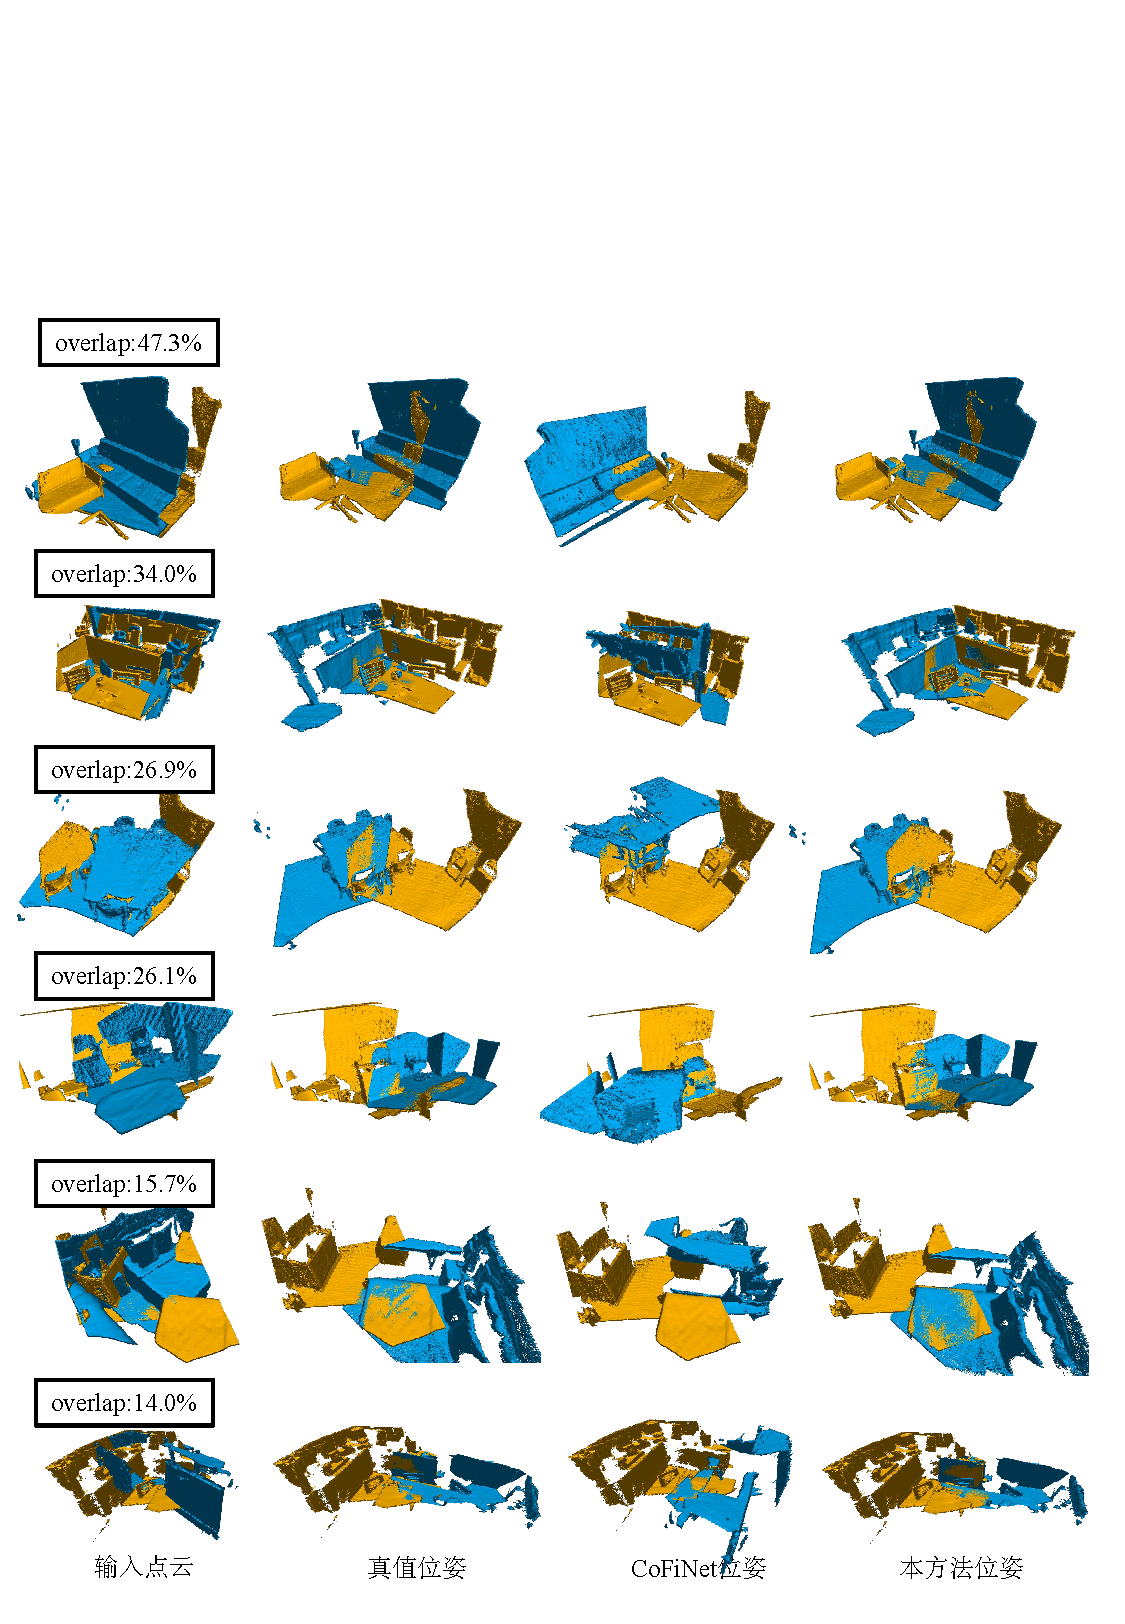
\includegraphics[width = \textwidth]{my/figure/4-4.pdf}
        \captionsetup{margin = {1.6cm,1.6cm}}
        \bicaption[\xiaosi 配准结果可视化]{\wuhao 配准结果可视化
        % 。(a) 输入点云;(b) 真实位姿;(c) CoFiNet位姿;(d) 本方法位姿
        }
        {\wuhao Visualization of registration results
        % . (a) Input; (b) Ground truth; (c) CoFiNet Pose; (d) Our Pose
        }
        \label{fig:4-4}
    \end{figure}
    \vspace{-0.35cm}

    \subsection{消融实验}
    本文提出的基于多模态融合的锚点定位点云配准方法为解决点云配准提供了一种新的思路,为了验证对齐模块和融合模块的有效性,本节将对这两个模块进行消融实验。

    \subsubsection{对齐模块的效果}表\ref{tab:4-5}展示了对齐模块的对本点云配准框架的作用,实验结果显示了超点匹配率、特征召回率、内点率和匹配召回率四个性能指标。从表\ref{tab:4-5}可以看出,在使用对齐模块之后所有的性能指标都得到了有效提高。这说明在多模态特征融合之前进行模态间的数据对齐,寻找点云中的点和图像中的像素的对应有助于更好的特征融合。
    \begin{table}[H]
    \renewcommand{\arraystretch}{1}
    \centering
    \bicaption[\xiaosi 对齐模块消融实验]{\wuhao 对齐模块消融实验}{\wuhao Ablation experiments of alignment module}\label{tab:4-5}
    \wuhao

    \begin{tabular}{lcccccccc}
    \toprule[1.5pt]
    \multicolumn{1}{c}{\multirow{2}{*}{Model}}
    & \multicolumn{4}{c}{3DMatch}
    & \multicolumn{4}{c}{3DLoMatch}
    \\ \multicolumn{1}{c}{}
    
    & PIR   & FMR   & IR   & RR   & PIR   & FMR   & IR    & RR
    \\ \hline
    w/o Alignment
    & 83.4  & 98.0  & 68.8 & 89.0 & 53.1  & 85.6  & 42.4  & 71.8  \\
    Ours
    & 85.4  & 98.0  & 70.2 & 90.6 & 51.4  & 87.6  & 41.2  & 73.1  \\
    \bottomrule[1.5pt]
    \end{tabular}
\end{table}

    \subsubsection{融合模块的效果}在特征融合过程中,与以往的特征融合方式不同,本方法在两个子空间将超点特征和它所对应的像素特征进行了融合,表\ref{tab:4-6}验证本融合方式的有效性。
    其中cFusion表示直接将点云特征与图像特征进行拼接,aFusion表示将点云和图像特征直接利用注意力进行融合,iFusion表示仅在模态无关子空间进行特征融合。
    \begin{table}[htp]
    \renewcommand{\arraystretch}{1}
    \centering
    \bicaption[\xiaosi 融合模块消融实验]{\wuhao 融合模块消融实验}{\wuhao Ablation experiment of fusion module}\label{tab:4-6}
    \wuhao
    
    \begin{tabular}{lcccccccc}
    \toprule[1.5pt]
    \multicolumn{1}{c}{\multirow{2}{*}{\songti\wuhao Model}}
    & \multicolumn{4}{c}{\songti\wuhao 3DMatch}
    & \multicolumn{4}{c}{\songti\wuhao 3DLoMatch}
    \\ \multicolumn{1}{c}{}

    & PIR   & FMR   & IR   & RR   & PIR   & FMR   & IR    & RR    \\ \hline
    {\songti\wuhao cFusion}
    & 82.7  & 97.6  & 68.3 & 87.8 & 48.5  & 84.5  & 39.3  & 69.7  \\
    {\songti\wuhao aFusion}
    & 83.4  & 97.6  & 68.6 & 88.8 & 49.5  & 83.9  & 39.7  & 70.3  \\
    {\songti\wuhao iFusion}
    & 84.4  & 97.8  & 70.1 & 89.9 & 51.8  & 85.8  & 42.2  & 72.2  \\
    {\songti\wuhao Ours}
    & 85.4  & 98.0  & 70.2 & 90.6 & 51.4  & 87.6  & 41.2  & 73.1  \\
    \bottomrule[1.5pt]
    \end{tabular}
\end{table}
    可以看到融合模块能够有效提高各个阶段的实验性能。这说明通过将两种模态特征投影到模态无关子空间能够有效减少模态间的域差异,同时在模态相关子空间的特征融合能够减少信息的丢失。

    \section{本章小结}
    本章提出了一个基于多模态特征融合的锚点定位点云配准方法,在第三章的基于锚点几何嵌入点云配准基础框架中的锚点定位阶段引入了多模态融合辅助定位。一方面,受到3D目标检测同行多模态融合方法的启发,该方法利用一个对齐模块寻找点云的点与图像的像素之间的对应关系,实现像素到点的准确映射。另一方面,该方法加入模态相关与无关的特征学习,旨在在模态无关子空间中减少模态间特征差异,同时利用注意力机制融合不同模态的信息,并在模态相关子空间中融合最终特征防止信息丢失。实验表明,本章提出的方法对如何融合点云和图像信息并最终受益于点云配准方法提供了很好的解决思路,同时提高了点云配准的性能。相比于其他方法,本方法在多模态融合之前进行了模态间的对齐,提升了多模态融合的效果,取得了更好的点云配准任务的实验结果。